\chapter{Implementación}

En este capítulo se mostraran los fundamentos mas importantes sobre la implementación tanto del front-end como del back-end y de como montar un instalador para Windows.

\subsection{Implementación del front-end}

En esta sección se explicaran cuales son las configuraciones más importantes de Angular.js porque este es el más importante del front-end. 

\subsubsection{Organización y carpetas}

La capeta public es la que contiene todo lo relacionado con el front-end del simulador de escenarios. Dento de este encontramos la siguiente estructura de directorios: 

\dirtree{%
	.1 Simulator.
	.2 public.
	.3 images.
	.3 javascript.
	.4 angular.
	.4 bootstrap.
	.4 jquery.
	.4 openlayers.
	.4 socketsIO.
	.3 stylesheets.
	.3 views.
}

A continuación vamos a ver cual es la función de cada uno de estos directorios:
\begin{itemize}
	\item images: contiene imágenes estáticas que se están utilizando en la aplicación.
	\item javascript: contiene todos los frameworks de javascript que se están utilizando en el front-end. Hay una carpeta para cada framework.
	\item javascript/angular: contiene todas las configuraciones de Angular.js. Este tiene 4 subdirectorios: config (contiene el router de Angular.js), controllers (contiene los controladores de Angular.sj), factory (contiene el factory de Angular.js) y services (contiene los servicios de Angular.js).
	\item javascript/bootstrap: contiene el sistema de componentes de bootstrap.
	\item javascript/openlayers: contiene el framework de OpenStreetMap.
\end{itemize}

\subsubsection{El router de Angular.js}

El router de Angular.js es el encargado del direccionamiento dentro de la página. En las configuraciones de este vinculamos una URL con una vista y esta con un controlador. Podemos encontrar las configuraciones de este en la carpeta /public/javascript/angular/config/routes.js:

\begin{lstlisting}[language=xml, frame=single]
var app = angular.module("app", ['ngRoute', 'ngStorage', 'checklist-model', 'xeditable']);

app.config(['$routeProvider', '$httpProvider' ,function($routeProvider, $httpProvider) {	 		   
$routeProvider.when('/', {
templateUrl: 'views/index.html',
controller: 'LoginController'
}).when('/register', {
templateUrl: 'views/register.html',
controller: 'RegisterController'
}).when('/map', {
templateUrl: 'views/maps/index.html',
controller: 'MapController'
}).when('/map/newMap', {
templateUrl: 'views/maps/newMap.html',
controller: 'NewMapController'        
}).when('/map/editScene', {
templateUrl: 'views/maps/editScene.html',
controller: 'EditSceneController'        
}).when('/map/editMap', {
templateUrl: 'views/maps/editMap.html',
controller: 'EditMapController'
}).when('/simulator', {
templateUrl: 'views/simulator/index.html',
controller: 'SimulatorController'
}).when('/settings', {
templateUrl: 'views//settings/recommenderSettings.html',
controller: 'RecommenderSettingsController'
}).when('/settings/staticItemSettings', {
templateUrl: 'views/settings/staticItemSettings.html',
controller: 'StaticItemSettingsController'
}).when('/settings/dynamicItemSettings', {
templateUrl: 'views/settings/dynamicItemSettings.html',
controller: 'DymanicItemSettingsController'
}).when('/profile', {
templateUrl: 'views/configurations/index.html',
controller: 'ConfigurationController'
}).otherwise({
redirectTo: '/'
}); 

$httpProvider.interceptors.push(['$q', '$location', '$localStorage', function($q, $location, $localStorage) {
return {  
'request': function (config) {    
config.headers = config.headers || {};

if ($localStorage.token) {
config.headers.Authorization = 'Bearer ' + $localStorage.token;
}

return config;

},

'responseError': function(response) {
if(response.status === 401 || response.status === 403) {
$location.path('/signin');
}

return $q.reject(response);
}
};    
}]);    
}]);
\end{lstlisting}

En el mismo fichero tenemos configurado también un interceptor. El interceptor es un método que se ejecuta cada vez que llega o sale una petición. En nuestro caso el interceptor es utilizado para encriptar y desencriptar los datos involucrados en la comunicación. También es el encargado de poner la cabecera Authorization que se utiliza para autentificar el usuario en cada petición.

\subsubsection{Los controladores de Angular.js}

Los controladores de Angular.js contienen la lógica de las vistas y establecen la comunicación con el back-end mediante los servicios de Angular.js. Existe un controlador por cada página y contiene funciones y datos propias de la vista. Como regla general se ha establecido que el nombre de controlador es el mismo que la vista a la que va asociada pero acabado con la palabra clave Controller. Podemos encontrar todos los controladores en la carpeta /public/javascript/angular/controllers.  

\begin{figure}[H]
	\centering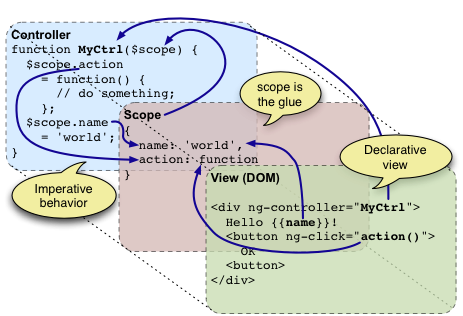
\includegraphics[scale=0.5]{imagenes/concepts-controller.png}
	\caption{Ejemplo de un controlador}
	\label{controllerExample}
\end{figure}

Según la filosofía de Angular.js las vista se actualizan de forma automática cuando actualizamos el modelo de datos del controlador. A continuación podemos ver un diagrama a cerca de como funciona:

\begin{figure}[H]
	\centering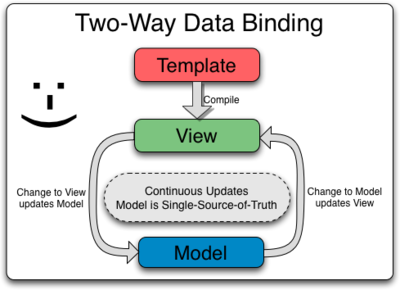
\includegraphics[scale=0.5]{imagenes/twoway.png}
	\caption{Two-way data binding}
	\label{twoWayDataBinding}
\end{figure}

\subsubsection{Los servicios de Angular.js}

Tener toda la lógica metida en los controladores y en el modelo de datos no es buena idea porque cuando la aplicación empieza a crecer se complican las cosas.

Los servicios son un concepto importante en Angular.js porque nos permiten agrupar funcionalidades que luego estarán disponible en los controladores, mejorando la claridad del código y favoreciendo la reutilización.

En nuestro caso hemos agrupado las llamadas al back-end y accedemos a la información del usuario autentificado desencriptada por los interceptores. Podemos encontrar todas las configuraciones de los servicios en el fichero /public/javascripts/angular/services/Services.js.

\subsection{Implementación del back-end}

En esta sección se explican cuales son las configuraciones más importantes de Node.js y Express. 

\subsubsection{Organización y carpetas}

El back-end se basa en la filosofía de desarrollo de aplicaciones con Node.js  Express. A continuación podemos ver cuales son los ficheros y directorios mas importantes:

\dirtree{%
	.1 Simulator.
	.2 app.js.
	.2 package.json.
	.2 routes.
	.3 configurations.js.
	.3 evaluation.js.
	.3 maps.js.
	.3 user.js.
	.2 models.
}

El primer fichero que vemos el app.js. Ahí es donde se encuentran todas las configuraciones del back-end como por ejemplo como se realiza el enrutamiento dento de la REST API, la conexión con la base de datos y las configuraciones de sockets.io.

El fichero package.json forma parte del gestor de paquetes npm y contiene todos los modulos que estamos usando en la aplicación. 

Por ultimo nos encontramos con los directorios routes y models. En el directorio routes podemos encontrar todo lo relacionado con el enrutamiento interno de la REST API y en models encontramos el modelo de datos usado en la base de datos.

\subsection{¿Cómo crear un instalador de la aplicación?}

Para crear un instalador de la aplicación se ha utilizado el programa Inno Setup v5.5.9. Dispone de un asistente de configuración que podemos ver en las secciones siguientes. Una vez que hayamos finalizado el asistente se crea un script que tenemos que compilar. Durante la complicación se comprimen todos los ficheros y directorios de nuestro proyecto y nos pide cual es el programa que tenemos que ejecutar cada vez que se inicie la aplicación.

\subsubsection{Pasos previos}

Para la aplicación pueda instalarse y ejecutarse como cualquier programa en Windows lo que necesitamos es que Maven, Node.js y mongoDB se nos instalen y configuren de forma automática con el instalador. El problema que esto supone es que el instalador no permite instalar programas externos porque lo único que haces es descomprimir el directorio de nuestra aplicación y crear un acceso directo para script que arranca los diferentes componentes del sistema: arrancar mongoDB, simulador y el recomendador. A continuación podemos ver el contenido del script que arrancar los distintos componentes del sistema:

\begin{lstlisting}[language=xml, frame=single]
@echo off
SET M2_HOME=../aplications/maven
SET M2=%M2_HOME%/bin
SET PATH=%M2%;%M2_HOME%

if "%PROCESSOR_ARCHITECTURE%" == "x86" ( 
SET PATH=%PATH%;aplications/mongodb32bits/bin;aplications/nodejs32bits;
) ELSE (
SET PATH=%PATH%;aplications/mongodb/bin;aplications/nodejs;
)

start mongod.exe --dbpath=aplications/data/db

start npm start

cd Recommender
start mvn exec:java -Dexec.mainClass=Server
cd ..
\end{lstlisting}

Para solucionar el problema de la instalación de programas externos se han incluido los programas externos en la carpeta aplications que se encuentra en el directorio raíz del simulador. En esta carpeta se han incluido Maven, Node.js y mongoDB. Hay que tener en cuenta que Node.js y mongoDB tienes distintas implementaciones para 32 y 64 bits. Por esto se han incluido ambas implementaciones en esta carpeta. Por esto durante el arranque se comprueba el tipo de sistema donde se este instalando el simulador y se configura en el PATH en función de esto.

Debido a que los programas externos disponen de ficheros demasiado grandes no era posible subirlos a ningún repositorio. Ademas que los repositorios de git no permite subir ejecutables por razones de seguridad. Por esto se han comprimido en un fichero .zip de fragmentado de 5MB cada fichero. Este fichero .zip fragmentado lo podemos encontrar dentro del directorio aplications y tenemos que descomprimirlo dentro de este directorio. 

El mismo problema ha surgido al subir el instalador en los repositorios Github y Gitlab. Por esto también se ha comprimido el instalador en un fichero .zip fragmentado. Podemos encontrarlo dentro del directorio instalador.

Una vez descomprimidos estos dos ficheros comprimidos podemos proceder a eliminarlos porque si hacemos un nuevo instalador estos ficheros se comprimirán dentro del nuevo instalador y este ocupará mucho más. 

\subsubsection{Paso 1}

En la primera pantalla solo vemos un texto informativo y lo único que tenemos que hacer es pulsar en Next:

\begin{figure}[H]
	\centering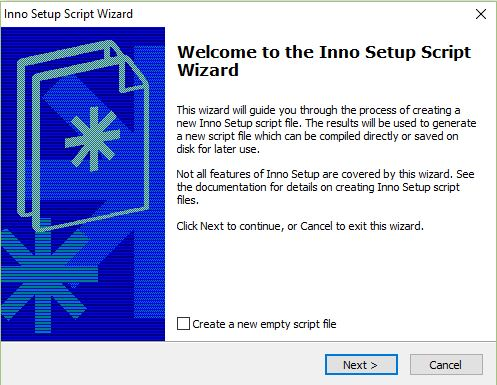
\includegraphics[scale=0.5]{imagenes/implementacion/1.jpg}
	\caption{Paso 1}
	\label{instaladorPaso1}
\end{figure}

\subsubsection{Paso 2}

En el segundo paso tenemos que rellenar un formulario con la siguiente información: el nombre de la aplicación, la versión e información de autor. 

\begin{figure}[H]
	\centering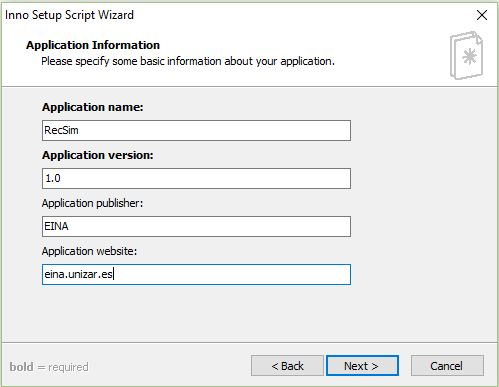
\includegraphics[scale=0.5]{imagenes/implementacion/2.jpg}
	\caption{Paso 2}
	\label{instaladorPaso2}
\end{figure}

\subsubsection{Paso 3}

En este paso indicamos cual es el nombre de la carpeta donde se van a descomprimir todos los ficheros tras la instalación:

\begin{figure}[H]
	\centering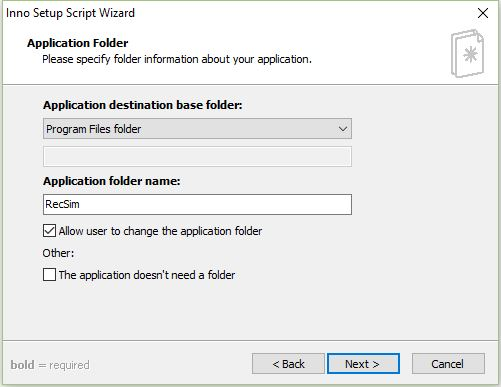
\includegraphics[scale=0.5]{imagenes/implementacion/3.jpg}
	\caption{Paso 3}
	\label{instaladorPaso3}
\end{figure}

\subsubsection{Paso 4}

En este paso tenemos que indicar cual es el script o ejecutable que arranca la aplicación e incluir el directorio del proyecto que sera comprimido en el instalador.

\begin{figure}[H]
	\centering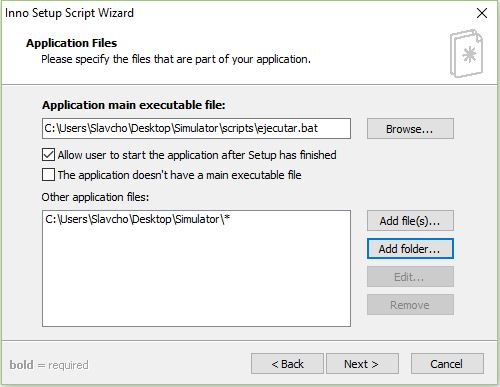
\includegraphics[scale=0.5]{imagenes/implementacion/4.jpg}
	\caption{Paso 4}
	\label{instaladorPaso4}
\end{figure}

\newpage

\subsubsection{Paso 5}

En este paso dejamos seleccionadas las opciones de crear un acceso directo en el menú de inicio e indicar que queremos un desinstalador:

\begin{figure}[H]
	\centering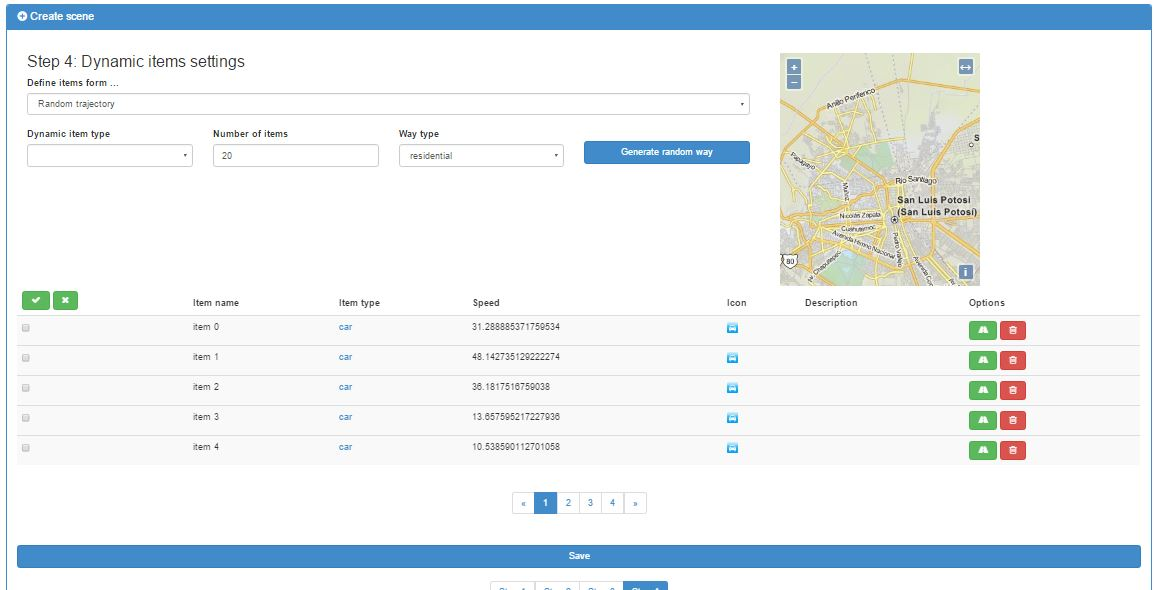
\includegraphics[scale=0.5]{imagenes/implementacion/5.jpg}
	\caption{Paso 5}
	\label{instaladorPaso5}
\end{figure}

\subsubsection{Paso 6}

En este paso disponemos de opciones de licencias de software. En nuestro caso las dejamos vacías:

\begin{figure}[H]
	\centering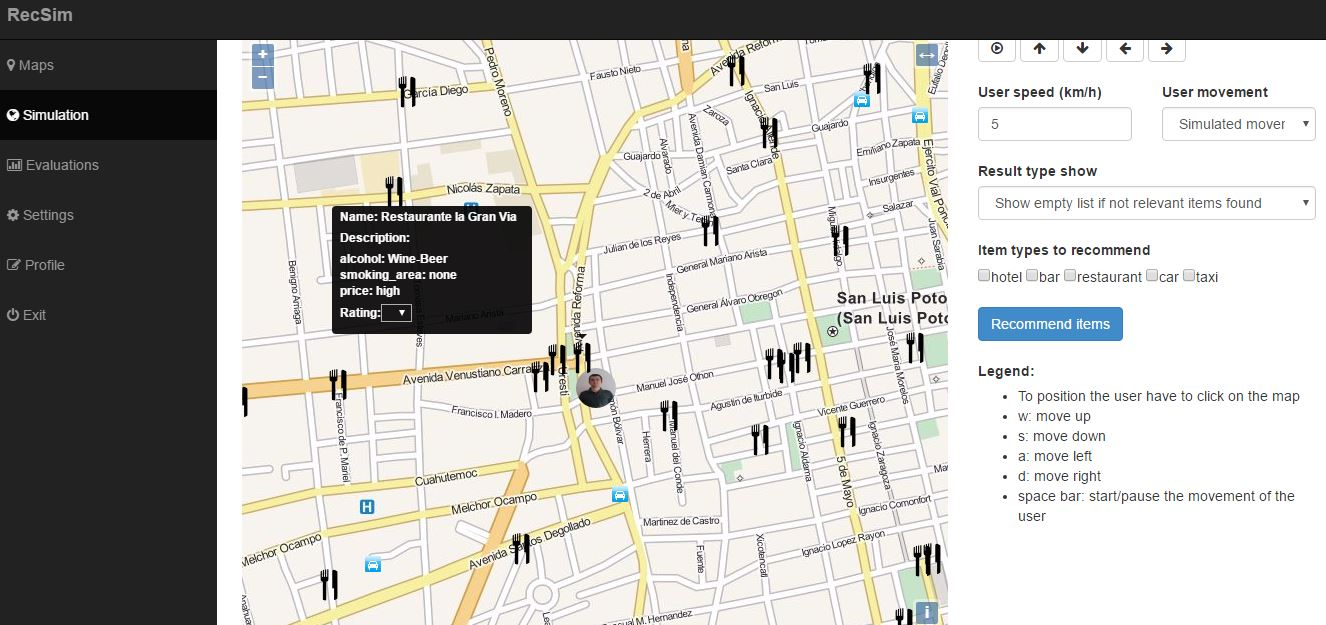
\includegraphics[scale=0.5]{imagenes/implementacion/6.jpg}
	\caption{Paso 6}
	\label{instaladorPaso6}
\end{figure}

\newpage

\subsubsection{Paso 7}

En este paso indicamos cuales son los idiomas que se nos mostraran durante la instalación. Los dejamos todos seleccionados:

\begin{figure}[H]
	\centering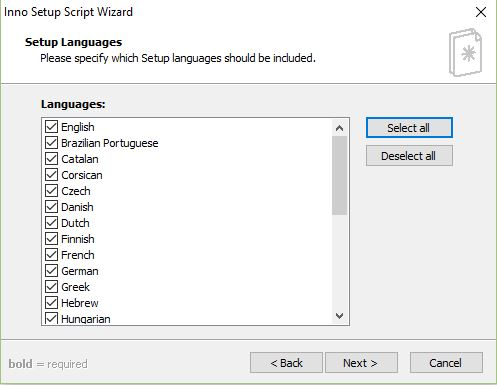
\includegraphics[scale=0.5]{imagenes/implementacion/7.jpg}
	\caption{Paso 7}
	\label{instaladorPaso7}
\end{figure}

\subsubsection{Paso 8}

En este paso tenemos que indicar cual es el directorio de salida donde se dejara el ejecutable, el nombre del instalador y su icono:

\begin{figure}[H]
	\centering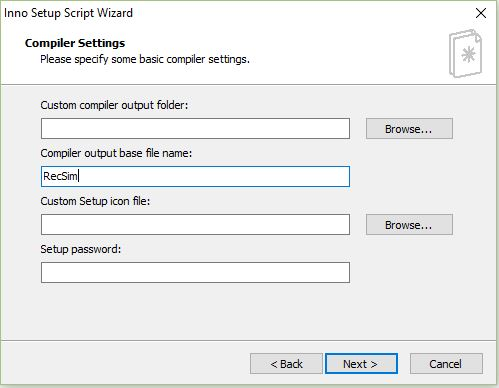
\includegraphics[scale=0.5]{imagenes/implementacion/8.jpg}
	\caption{Paso 8}
	\label{instaladorPaso8}
\end{figure}

\newpage

\subsubsection{Paso 9}

En este paso nos preguntan si queremos incluir directivas en el script que se nos va a crear. Estas directivas tienen la función de variables globales con información que se reutiliza en el script como por ejemplo el nombre del instalador etc. En este caso dejamos el check marcado:

\begin{figure}[H]
	\centering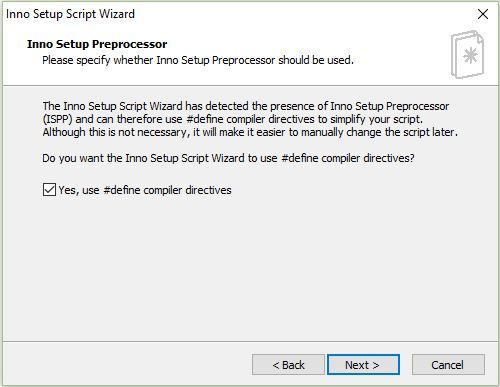
\includegraphics[scale=0.5]{imagenes/implementacion/9.jpg}
	\caption{Paso 9}
	\label{instaladorPaso9}
\end{figure}

\subsubsection{Paso 10}

Este el ultimo paso y lo único que tenemos que hacer es pulsar en Finish para finalizar el asistente:

\begin{figure}[H]
	\centering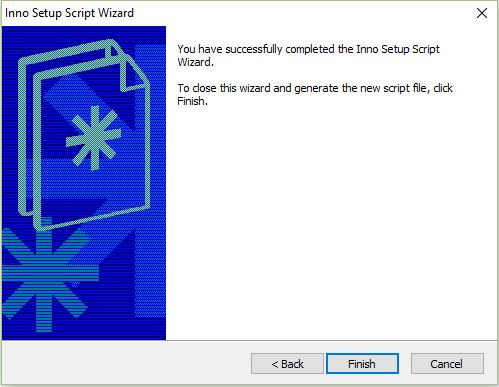
\includegraphics[scale=0.5]{imagenes/implementacion/10.jpg}
	\caption{Paso 10}
	\label{instaladorPaso10}
\end{figure}

\newpage

Observamos que se genera un script como este:

\begin{lstlisting}[language=xml, frame=single]
; Script generated by the Inno Setup Script Wizard.
; SEE THE DOCUMENTATION FOR DETAILS ON CREATING INNO SETUP SCRIPT FILES!

#define MyAppName "Simulator"
#define MyAppVersion "1.0"
#define MyAppPublisher "EINA"
#define MyAppURL "eina.unizar.es"
#define MyAppExeName "ejecutar.bat"

[Setup]
; NOTE: The value of AppId uniquely identifies this application.
; Do not use the same AppId value in installers for other applications.
; (To generate a new GUID, click Tools | Generate GUID inside the IDE.)
AppId={{23676D0A-DCBC-41E5-B959-47753F7EE277}
AppName={#MyAppName}
AppVersion={#MyAppVersion}
;AppVerName={#MyAppName} {#MyAppVersion}
AppPublisher={#MyAppPublisher}
AppPublisherURL={#MyAppURL}
AppSupportURL={#MyAppURL}
AppUpdatesURL={#MyAppURL}
DefaultDirName={pf}\{#MyAppName}
DefaultGroupName={#MyAppName}
DisableProgramGroupPage=yes
OutputBaseFilename=Simulator
Compression=lzma
SolidCompression=yes
AlwaysShowDirOnReadyPage=yes

[Languages]
Name: "english"; MessagesFile: "compiler:Default.isl"
Name: "brazilianportuguese"; MessagesFile: "compiler:Languages\BrazilianPortuguese.isl"
Name: "catalan"; MessagesFile: "compiler:Languages\Catalan.isl"
Name: "corsican"; MessagesFile: "compiler:Languages\Corsican.isl"
Name: "czech"; MessagesFile: "compiler:Languages\Czech.isl"
Name: "danish"; MessagesFile: "compiler:Languages\Danish.isl"
Name: "dutch"; MessagesFile: "compiler:Languages\Dutch.isl"
Name: "finnish"; MessagesFile: "compiler:Languages\Finnish.isl"
Name: "french"; MessagesFile: "compiler:Languages\French.isl"
Name: "german"; MessagesFile: "compiler:Languages\German.isl"
Name: "greek"; MessagesFile: "compiler:Languages\Greek.isl"
Name: "hebrew"; MessagesFile: "compiler:Languages\Hebrew.isl"
Name: "hungarian"; MessagesFile: "compiler:Languages\Hungarian.isl"
Name: "italian"; MessagesFile: "compiler:Languages\Italian.isl"
Name: "japanese"; MessagesFile: "compiler:Languages\Japanese.isl"
Name: "norwegian"; MessagesFile: "compiler:Languages\Norwegian.isl"
Name: "polish"; MessagesFile: "compiler:Languages\Polish.isl"
Name: "portuguese"; MessagesFile: "compiler:Languages\Portuguese.isl"
Name: "russian"; MessagesFile: "compiler:Languages\Russian.isl"
Name: "scottishgaelic"; MessagesFile: "compiler:Languages\ScottishGaelic.isl"
Name: "serbiancyrillic"; MessagesFile: "compiler:Languages\SerbianCyrillic.isl"
Name: "serbianlatin"; MessagesFile: "compiler:Languages\SerbianLatin.isl"
Name: "slovenian"; MessagesFile: "compiler:Languages\Slovenian.isl"
Name: "spanish"; MessagesFile: "compiler:Languages\Spanish.isl"
Name: "turkish"; MessagesFile: "compiler:Languages\Turkish.isl"
Name: "ukrainian"; MessagesFile: "compiler:Languages\Ukrainian.isl"

[Tasks]
Name: "desktopicon"; Description: "{cm:CreateDesktopIcon}"; GroupDescription: "{cm:AdditionalIcons}"; Flags: unchecked

[Files]
Source: "C:\Users\Slavcho\Desktop\Simulator\scripts\ejecutar.bat"; DestDir: "{app}"; Flags: ignoreversion
Source: "C:\Users\Slavcho\Desktop\Simulator\*"; DestDir: "{app}"; Flags: ignoreversion recursesubdirs createallsubdirs
; NOTE: Don't use "Flags: ignoreversion" on any shared system files

[Icons]
Name: "{group}\{#MyAppName}"; Filename: "{app}\{#MyAppExeName}"
Name: "{group}\{cm:ProgramOnTheWeb,{#MyAppName}}"; Filename: "{#MyAppURL}"
Name: "{group}\{cm:UninstallProgram,{#MyAppName}}"; Filename: "{uninstallexe}"
Name: "{commondesktop}\{#MyAppName}"; Filename: "{app}\{#MyAppExeName}"; Tasks: desktopicon

[Run]
Filename: "{app}\{#MyAppExeName}"; Description: "{cm:LaunchProgram,{#StringChange(MyAppName, '&', '&&')}}"; Flags: shellexec postinstall skipifsilent
\end{lstlisting}
